\documentclass[11pt,a4paper]{article}
\usepackage{amsmath,amsthm}
\usepackage{tikz,pgfplots}

\begin{document}

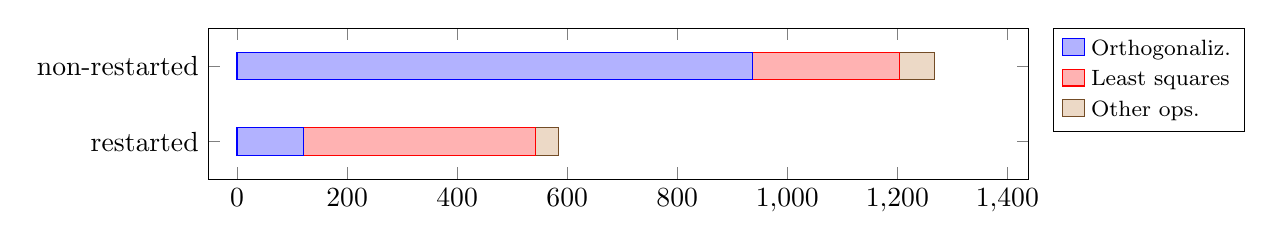
\begin{tikzpicture}
       \begin{axis}[
           xbar stacked,
           enlargelimits=0.15,
           legend pos=outer north east,
           legend cell align={left},
           legend style={font=\footnotesize},
           width=12cm, height=3.5cm, enlarge y limits=0.5,
           symbolic y coords={restarted, non-restarted},
           ytick=data,
       ]
        % 0 = restarted (ncv=40, nconv=20) time=5.8553e+02 orthogonalize=1.2038e+02 KSPSolve=4.2237e+02
        % 1 = non-restarted (ncv=765, nconv=22) time=1.2676e+03 orhogonalize=9.3643e+02 KSPSolve=2.6832e+02
        \addplot coordinates {  % bvorthogonalize
            (120,restarted) (936,non-restarted)
        };
        \addplot coordinates {  % kspsolve
            (422,restarted) (268,non-restarted)
        };
        \addplot coordinates {  % rest
            (43,restarted) (62.8,non-restarted)
        };
        \legend{Orthogonaliz.,Least squares,Other ops.}
    \end{axis}
    \end{tikzpicture}

\end{document}